
\section{dinamica complessa}
\label{sec:mandelbrot}
\index{dinamica!complessa}

Più in generale potremmo considerare successioni $z_n$ a valori complessi
e quindi equazioni ricorsive della forma
\[
  \begin{cases}
    z_0 = \alpha, \\
    z_{n+1} = f(z_n)
  \end{cases}
\]
con $f\colon \CC \to \CC$.
Se $f$ fosse lineare si potrebbe scrivere esplicitamente la soluzione
seguendo le idee presentate nella sezione~\ref{sec:ricorrenza_lineare}.

Possiamo provare a considerare la più semplice funzione non lineare che ci possa
venire in mente cioè $f(z) = z^2 + c$ e il più semplice dato iniziale $\alpha = 0$
e il problema diventa quello di studiare il comportamento delle successioni:
\begin{equation}\label{eq:mandelbrot}
  \begin{cases}
    z_0 = 0, \\
    z_{n+1} = z_n^2 + c
  \end{cases}
\end{equation}
con $c\in \CC$.

L'insieme dei numeri reali è invariante, dunque se $c\in \RR$ la successione
$z_n$ rimane reale e coincide con la successione che abbiamo
studiato nell'esercizio~\ref{ex:mandelbrot_reale}.

\begin{figure}
\begin{center}
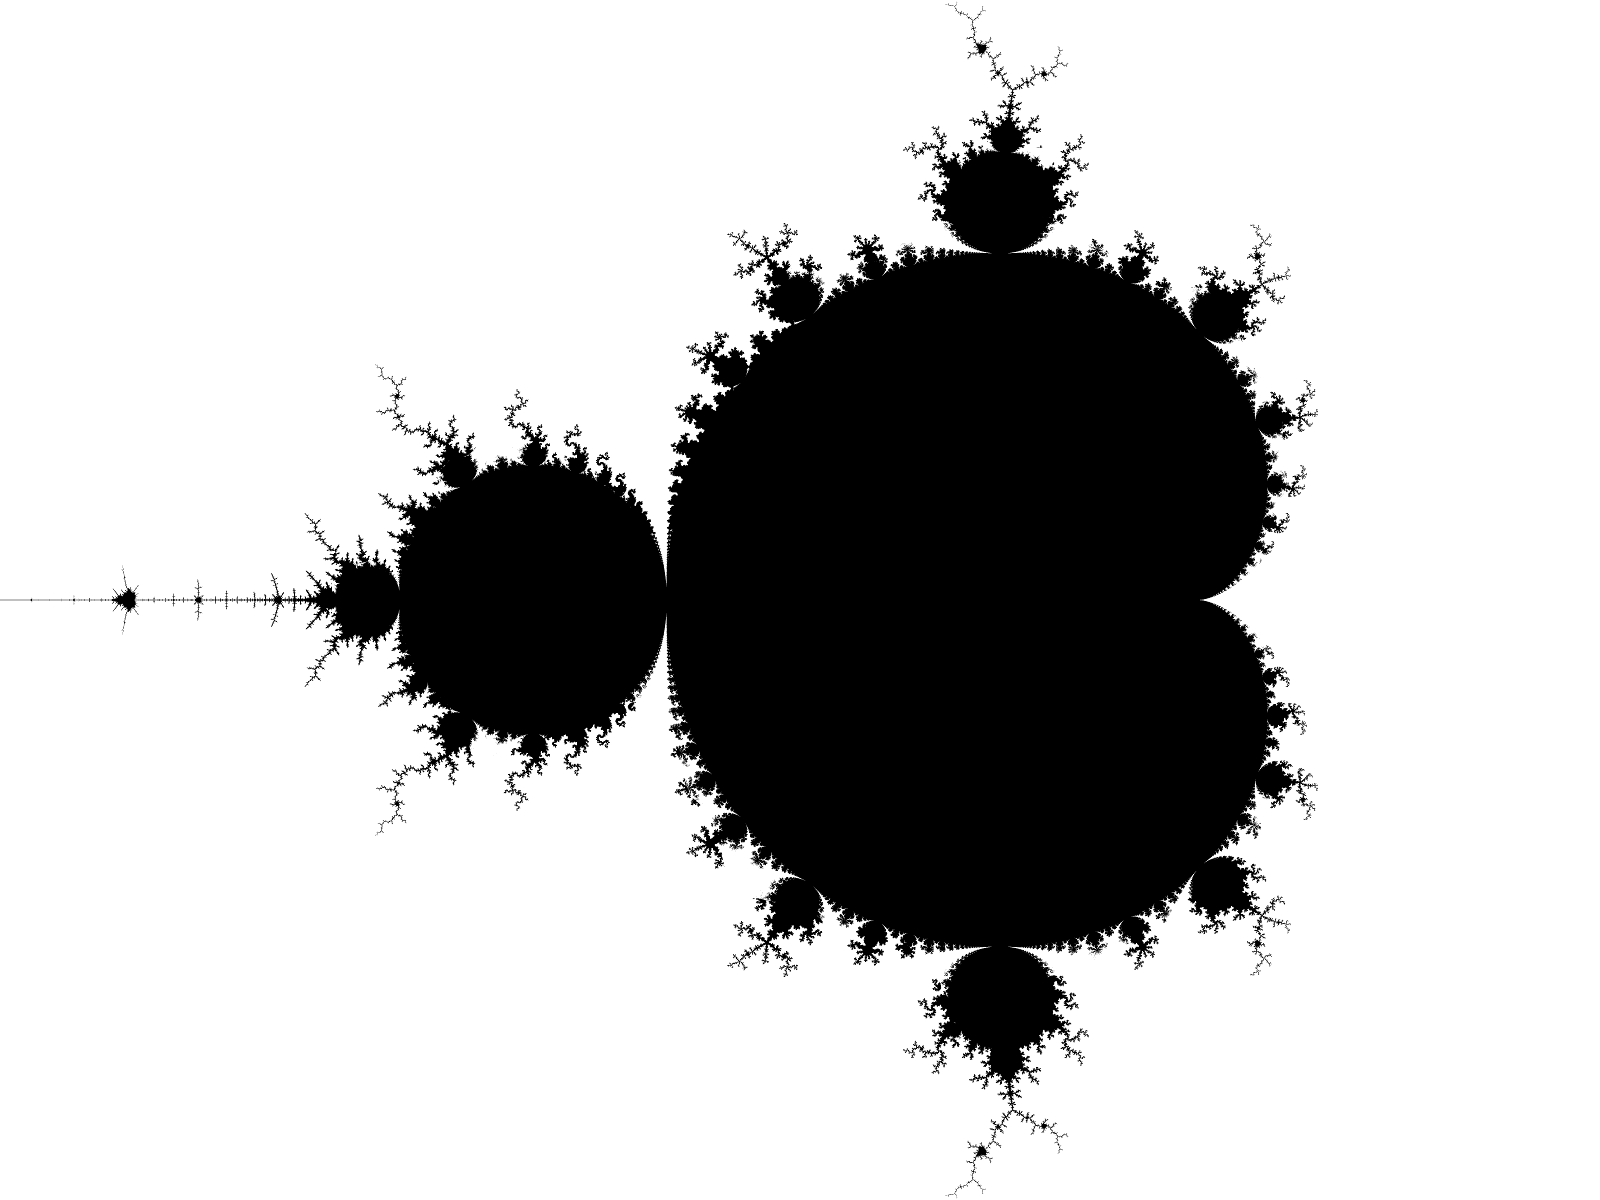
\includegraphics[width=\textwidth]{mandelbrot.png}
\end{center}
\caption{L'insieme di Mandelbrot generato al computer. Si veda il
codice a pagina \pageref{code:Mandelbrot}.}
\label{fig:mandelbrot}
\end{figure}

E' molto complicato determinare il carattere delle successioni definite
dal sistema~\eqref{eq:mandelbrot}.
Solo con l'utilizzo dei primi calcolatori
Mandelbrot (1924-2010) riuscì a rappresentare graficamente
\mymargin{insieme di Mandelbrot}%
\index{insieme!di Mandelbrot}%
\index{Mandelbrot!insieme di}%
l'insieme $M$ dei punti $c\in \CC$ per i quali la successione $z_n$ non diverge:
si veda la figura~\ref{fig:mandelbrot}.

Con l'esercizio~\ref{ex:mandelbrot_reale}
abbiamo trovato l'intersezione $M\cap \RR = [-2,1/4]$.
Nel seguente esercizio ci proponiamo ora di dimostrare un'altra semplice
proprietà che può essere
molto utile negli algoritmi numerici utilizzati per disegnare tale insieme.

\begin{exercise}[raggio di fuga]
Dimostrare che se $z_n$ è soluzione di \eqref{eq:mandelbrot}
se per un qualche $N\in \NN$ si ha $\abs{z_N}> 2$ allora $\abs{z_n}\to +\infty$
per $n\to +\infty$. In particolare l'insieme $M$ di Mandelbrot
è contenuto nel disco $\ENCLOSE{z\in \CC \colon \abs{z}\le 2}$.
\end{exercise}
%
\begin{proof}[Soluzione]
Sia $c\in \CC$ fissato e si $z_n$ la successione definita da~\eqref{eq:mandelbrot}.
Per ogni $\eps>0$ consideriamo l'insieme:
\[
  A_\eps = \ENCLOSE{z \in \CC \colon \abs{z}\ge c \text{ e } \abs{z}\ge 2+\eps}.
\]
Possiamo mostrare che l'insieme $A_\eps$ è invariante in quanto se $z_n\in A_\eps$
si ha
\begin{equation}\label{eq:473244}
\begin{aligned}
\abs{z_{n+1}}
&= \abs{z_n^2+c}
\ge \abs{z_n}^2 - \abs{c}
\ge \abs{z_n}^2 - \abs{z_n}
= (\abs{z_n}-1)\abs{z_n}\\
&\ge (1+\eps)\abs{z_n}
\ge (1+\eps)(2+\eps)
\ge 2+\eps.
\end{aligned}
\end{equation}
Dunque $A_\eps$ è invariante ma non solo, se $z_n \in A_\eps$ abbiamo
trovato che risulta $\abs{z_{n+1}} \ge (1+\eps) \abs{z_n}$
e dunque $\abs{z_{n+k}} \ge (1+\eps)^k \abs{z_n}$ e dunque
$\abs{z_n}\to +\infty$ per $n\to +\infty$.

Se $\abs{c}\le 2$ e se $\abs{z_N}> 2$ allora $z_N \in A_\eps$ per
un qualche $\eps>0$ e dunque possiamo concludere che
$z_n\to \infty\in \bar \CC$.
Se invece $\abs{c}>2$ è facile osservare che $z_0 = 0$, $z_1=c$, $z_2=c^2+c$
e quindi
\[
  \abs{z_2}
    = \abs{c^2+c}
    \ge \abs{c}^2 - \abs{c}
    = \abs{c}(\abs{c}-1)
    \ge \abs{c} > 2
\]
dunque $z_2 \in A_\eps$ e quindi, comunque, $z_n\to \infty$.

\end{proof}
